\newpage
%%%%%%%%%%%%%%%%%%%%%%%%%%%%%%%%%%%%%%%%%%%%%%%
%%%%%%%%%%%%%%%%%%%%%%%%%%%%%%%%%%%%%%%%%%%%%%%
%%%%%%%%%%%%%%%%%%%%%%%%%%%%%%%%%%%%%%%%%%%%%%%
\setcounter{section}{1}\section{国際SKAの科学的課題}
\label{c06.s2}

この節では、国際SKAサイエンスブックに掲載予定の宇宙磁場研究についてまとめる。

%%%%%%%%%%%%%%%%%%%%%%%%%%%%%%%%%%%%%%%%%%%%%%%
%%%%%%%%%%%%%%%%%%%%%%%%%%%%%%%%%%%%%%%%%%%%%%%
\subsection{国際SKAサイエンスの概要}
\label{c06.s2.ss1}

%%%%%%%%%%%%%%%%%%%%%%%%%%%%%%%%%%%%%%%%%%%%%%%
\subsubsection{科学的課題}
\label{c06.s2.ss1.sss1}

\paragraph{論文リスト}

国際SKA科学検討班が取りまとめた中で、本節では以下の論文を解説する。
\begin{itemize}
\item {\bf 全天RMグリッド:} SKAによる宇宙磁場研究の中核である。全天の電波源を捜査し、多数のRM観測点を得る。そのカタログを様々な宇宙磁場研究に役立てる。
\item {\bf 深探査:} 広視野を確保しながら従来より一桁以上向上した75 nJyのRMSの観測をSKA1で達成する。銀河やAGNの宇宙論的進化と、銀河間磁場の発見を狙う。
\item {\bf 広帯域観測:} RMグリッドと相補的でありながら、さらに数万の偏波銀河を非常に広帯域で観測する。広帯域の偏波特性を見ることで、空間分解に頼らずに偏波源周囲のプラズマ構造の特性と宇宙論的進化を理解する。
\item {\bf 天の川銀河:} 系外ソースのRMグリッド、パルサーの信頼できる距離とRM、そして広がったシンクロトロン放射の分光観測から、個別の前景天体を定め、円盤磁場モデルを精密化し、銀河中心の磁場を調査し、そして星間磁気乱流を特徴づける。
\item {\bf 系外銀河:} 星間磁場の小構造をマッピングして冷たいガスと磁場の結合やどのようにガス運動が影響されるか理解する。パワースペクトルから乱流磁場の起源と役割を知る。ハロー場の観測から宇宙線の輸送を検証し銀河流出の起動・放出・調整機構を探る。磁場構造を平均場ダイナモ理論と比較し、銀河ダイナモの増幅と飽和過程を特定する。
\item {\bf 近傍銀河のファラデートモグラフィ:} 分解能内の磁場やガス構造は繊細に波長に依存しながら偏波特性を変える。優れた感度と分解能に加え広帯域によりRM Synthesisなどの新しい手法を用いて、詳細なモデルとの比較からISMの物理構造を探る。
\item {\bf AGNジェット:} 広視野・高感度にSKA-VLBIの高分解能によって相対論的ジェットと星形成銀河を区別しながら円偏波もとらえて大量の近傍ジェットカタログを得る。再電離期まで遡る宇宙論的なジェット進化、ジェット構成物、radio loud/quietの二分、ジェットの3次元構造の特徴、ジェット周辺物質、ジェットと周辺物質と相互作用を解明する。
\item {\bf RMで探る銀河団:} 背景偏波源のRM観測データを使って、磁場の強度や構造、質量による違い、進化の異なるステージによる違い、宇宙論的進化を示す。衝突銀河団の衝撃波での磁場強度に制限をつける。
\item {\bf 電波ハローで探る銀河団:} シンクロトロン電波ハローから銀河団の磁場の性質を制限し、相対論的粒子の加速や輸送の物理に基礎的な制限を導く。
\item {\bf RMのスタック解析:} スタックした偏波を適用して、宇宙論的時間の関数での偏波解消、低光度ソースの磁場特性、平均的な磁場の向きと観測量との潜在的な相関を探る。
\end{itemize}
これら以外にも、「分子雲があるところのシンクロトロン放射」「ゼーマン効果で探る磁場」「電波銀河のkpcスケールジェットの運動学とダイナミクス」「環境探針としての広がった電波銀河」「低密度領域の大スケール磁場」「銀河フィラメント(電波放射)」「銀河フィラメント(RM)研究の統計的手法」「暗黒物質の研究」が提案されている。

%%%%%%%%%%%%%%%%%%%%%%%%%%%%%%%%%%%%%%%%%%%%%%%
\subsubsection{観測の見通し}
\label{c06.s2.ss1.sss2}

\begin{figure}[tbp]
\begin{center}
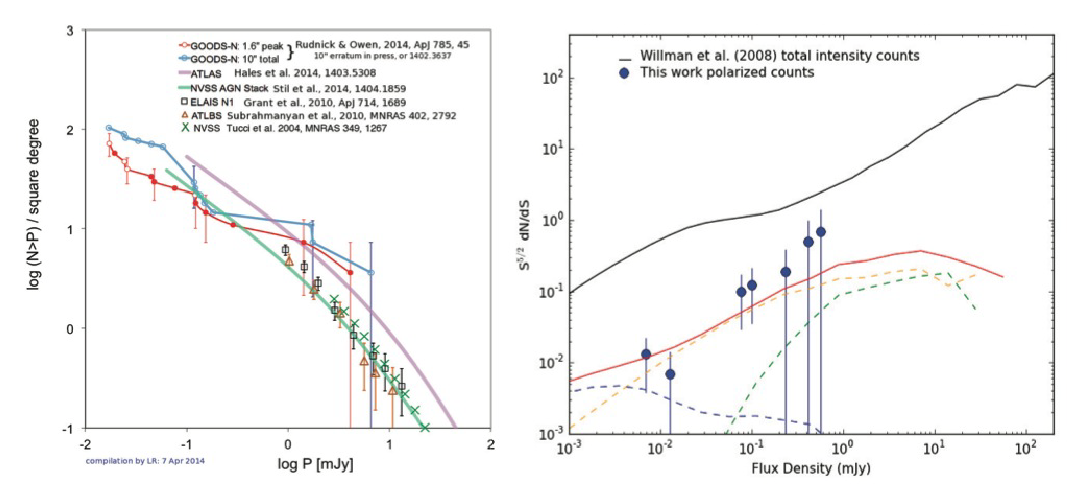
\includegraphics[width=0.95\linewidth]{magnetism/c06.s2.ss1.f1.eps}
\end{center}
\caption{左図:1.4 GHzでの様々な観測による15$\mu$Jyまでの積分偏波源数のまとめ \citep{Rudnick_private}。赤と青線は、VLAのGOODS-N視野(約0.2平方度)の深観測から見つかった偏波源を元にした推定\citep{2014ApJ...785...45R}で、紫はATCAのATLAS視野(約6平方度)の深観測から見つかった偏波源を元にした推定\citep{2014MNRAS.440.3113H}。緑はVLA-NVSSの浅い全天観測をスタックした推定\citep{2014ApJ...787...99S}。右図:JVLA 5 GHzでの5$\mu$Jyまでの微分偏波源カウント(点)とAGNならびに銀河のモデル(線)との比較 \citep{1405.0117}。緑、オレンジ、青の点線はそれぞれFR-II電波銀河, FR-I電波銀河, 星形成銀河の寄与。
}\label{c06.s2.ss1.f1}
\end{figure}

\paragraph{観測されたRMグリッド数}

図\ref{c06.s2.ss1.f1}左には1.4 GHzにおける15$\mu$Jyまでの偏波源数曲線を示す。結果にばらつきがあるが、2004年の推定に比べて数の伸びがゆるやかである。例えばASKAP POSSUMは、当初100 $\mu$Jy以上の偏波源が平方度あたり100体と想定していたが、それよりも現実はやや少ないかもしれない。

\paragraph{予想されるRMグリッド数}

図\ref{c06.s2.ss1.f1}左から悲観的に見積もると、10 $\mu$Jy以上の偏波源で平方度あたり100体、100 nJy以上の偏波源まで考えて平方度あたり1000体に達する。これらの数の偏波源を10$\sigma$で得るには、ポインティングあたり、前者はSKA1-MID(0.5平方度)で1時間またはSKA1-SUR(18平方度)で16時間の観測、後者はSKA1の10倍感度と仮定したSKA2-MIDで50時間の観測が必要である。もう少し現実的には、1 $\mu$Jy以上の偏波源は$1''$-$10''$の分解能の観測\citep{2014ApJ...785...45R, 2014MNRAS.440.3113H}に基づくと平方度あたり300体程度、$1'$の分解能の観測\cite{2014ApJ...787...99S}に基づくと平方度あたり1300体程度と見積もられている\citep{Cosmic_Magnetism_memo_2014}。実に因子4も不定性がある。図\ref{c06.s2.ss1.f1}右には5GHzでの5$\mu$Jyまでの偏波源数を示し、どの天体の寄与がどの程度あるかの予想も示す。これをみると、星形成銀河の集団がまさにこれからの観測の時代($10\mu$Jy以下)に新たに加わってくることが見て取れる。100 $\mu$Jy以下の淡い電波源は星形成銀河の他に、ULIRGsや衝突銀河、またおとなしい円盤銀河も期待される。これらの増分を考えると、上記の想定よりは多い偏波源が観測されるのかもしれない。結局のところは観測してみなければわからないわけで、この強度関数自体の調査も宇宙の天体形成を知る興味深いテーマである。


%%%%%%%%%%%%%%%%%%%%%%%%%%%%%%%%%%%%%%%%%%%%%%%
%%%%%%%%%%%%%%%%%%%%%%%%%%%%%%%%%%%%%%%%%%%%%%%
\subsection{星間・天の川銀河磁場}
\label{c06.s2.ss2}

%%%%%%%%%%%%%%%%%%%%%%%%%%%%%%%%%%%%%%%%%%%%%%%
\subsubsection{科学的課題}
\label{c06.s2.ss2.sss1}

\paragraph{大局磁場}

ダイナモ理論によると、銀河円盤では軸対称で銀河面に対して偶パリティ(銀河面に平行な磁場の成分は銀河面に対して同じ向きで、銀河面に垂直な磁場の成分は向きを変化させる)のモードが成長しやすい\citep{1988Natur.336..341R}。磁場は回転方向の成分が支配的で、それに動径成分が加わり、軸対称な渦構造を形成する。この形状、例えば左右相称(Bisymmetric)の磁場構造など、からのずれは他の銀河や棒状構造からの擾乱によるものかもしれない。一方、銀河ハローのような球形の構造を持った天体では軸対称で奇パリティ(偶パリティの逆)のモードが成長しやすく、円盤とハローが共存する系では偶パリティと奇パリティが混ざった結果が得られる可能性がある。実際にはどちらかのパリティが顕在化するという研究があるが\citep{2008A&A...487..197M}、銀河風が存在するため事情は複雑である。現在の観測は銀河磁場のダイナモモデルと矛盾はない。しかし、実際に銀河磁場がどのように維持されているのかを決めるのは困難である。

\paragraph{円盤磁場}

円盤内にある大局磁場は、渦状腕に沿った構造で、その強さはおよそ3 $\mu$Gである。最近のモデルでは、太陽より銀河中心側で一回だけ磁場が反転しているとされている\citep{2007ApJ...663..258B, 2008A&A...477..573S, 2011ApJ...728...97V, 2012ApJ...757...14J}。しかし、複数回の反転を結論づけている研究もある\citep{2006ApJ...642..868H, 2010A&A...513A..65N}。この磁場の反転構造は軸対称な磁場を持つ系外銀河では観測されていない。

\paragraph{乱流磁場}

銀河の星間ガスは電離ガスも中性ガスも乱流的であり、普通は密度に対してコルモゴロフのようなベキ乗型のパワースペクトルを示している\citep{2004ARA&A..42..211E, 1995ApJ...443..209A}。しかし、磁場は間接的な観測しかないため、磁場のパワースペクトルを測定するのは難しい。この星間乱流の平均的なマッハ数$M$は、$M \la 2$程度と見積もられている\citep{2014A&A...566A...5I}。また、乱流のエネルギー注入のスケールは、渦状腕では 1 pc のオーダー、渦状腕と渦状腕の間では 100 pc のオーダーであると見積もられている\citep{2008ApJ...680..362H}。さらに、密度の高いガスの星間乱流が間欠性を示すという複数の観測事実がある\citep{2004ARA&A..42..211E}。すなわち、強い乱流を示す領域と乱流を示さない領域がある。

\paragraph{ハロー磁場}

ハローに関しては偶と奇が混ざったパリティの構造を持つモデルが最もよさそうである \citep{2001MNRAS.325..649F, 2008A&A...477..573S, 2012ApJ...757...14J}。しかし、銀河ハローの磁場は銀河内の局所的な前景の影響を受けるため、現在の観測では困難である。

\paragraph{銀河中心磁場}

銀河中心の磁場はガスや相対論的粒子との相互作用により複雑である。そのため強さや構造には大きな不定性がある。最小エネルギーの見積もりからは$\sim (6-22)~\mu$G、シンクロトロン放射スペクトルからは$\sim (50-120)~\mu$G、磁場とガスの圧力バランスからは$\sim 1$~ mGである。マグネター(J1745-2900)のRMとDMを使った見積もりでは、Sgr A* から$\sim 0.1$~pc離れたところで $\sim 5-6$~mGである。高密度ガスのゼーマン効果やサブミリ波の偏波観測からは、0.1~mG から数~mGであった。構造については、銀河の力学中心から$\sim 50$~pc離れたところを中心にポロイダル磁場が$\sim 300$~pc にわたって存在しているという報告がある\citep{2003ApJ...583L..83N, 2011ApJ...731...36L}が、相反する研究結果もある。

\paragraph{星形成領域の磁場}

原始星ジェットの密度や温度や電離度は輝線放射の観測からよい制限がついているが、磁場の観測は間接的でモデルに依存している。原始星ジェットの非熱的放射は磁場に関する直接的な証拠を与えるが、非熱的放射は微弱でその観測はまれである。観測的には直接的な証拠はないが、ジェット形成における磁場の役割は、ガス円盤から中心星への活動的な降着流やその周囲にある分子雲と密接に関係し、磁気遠心力を介したジェットのMHD加速メカニズムは原始星ジェットの加速メカニズムとして広く受け入れられている。

\paragraph{超新星残骸の磁場}

超新星残骸の磁場はミリガウスにまで増幅されうる。若い超新星残骸の磁場は一般に動径方向を向いているが、古い超新星残骸の磁場は接線方向を向いていることが知られている。超新星残骸の磁場の重要性とは別に、超新星残骸は宇宙線の加速にとって欠く事ができない物である。また超新星残骸は銀河の大局磁場からも影響を受けている。超新星残骸の磁場が、銀河磁場やまたは元の星や星風の磁場をどのように反映しているのかはまだよくわかっていない。その問題を解決するためには、より多くのサンプルを分解して観測する必要がある。

\paragraph{HII領域の磁場}

HII領域の典型的な磁場の強さは数 $\mu$ Gから12 $\mu$ Gで\citep{2007A&A...463..993S, 2010A&A...515A..64G, 2011ApJ...736...83H}、背景偏波源のファラデー回転の観測から得られている。HII領域の磁場の測定を大きく異なる密度において行う事は磁場が力学的な役割を理解する上で必要であり、これは、より高密のRMグリッドによって調べる事が可能になる。

\paragraph{星雲の磁場}

パルサー風星雲とは、磁化された粒子がパルサーから供給されることによって生じた膨張する星雲であるが、その進化についてはよくわかっていない。理論モデルはあるが、理論モデルをテストするための観測例は少ない。惑星状星雲では、最近になって偏波が発見された。惑星状星雲そのものは磁場を持たないので、これは周囲の磁場が圧縮されたために違いない。ゆえに、惑星状星雲の偏波のマップは銀河の大局磁場を探査するのに役立つだろう。

\paragraph{ファラデースクリーン}

最後に、偏波観測から得られる構造で対応天体を同定することが困難なファラデースクリーンと呼ばれるものもある。それらの多くは連続光ではとても暗いが、偏波観測やRMでは明るく見える。ある物はパルサー風星雲か、または膨張する磁気バブルから離れている古いHII領域に関係しているかもしれないが、一般にその性質や起源はいまだに謎である。


%%%%%%%%%%%%%%%%%%%%%%%%%%%%%%%%%%%%%%%%%%%%%%%
\subsubsection{観測の見通し}
\label{c06.s2.ss2.sss2}

\paragraph{SKA1の見通し}

SKA1の高分解能の観測で星形成領域の非熱的な電波放射を解明することができる。原始星の降着円盤とジェット、星形成のMHDモデルと銀河磁場との関係などを探ることができる。現段階でどのくらい観測可能な天体があるのかを見積もる事はできないが、わずかな観測例でも観測されれば大きなインパクトを与える事になる。SKA1の高感度・広帯域・広視野の観測では、超新星残骸、HII領域、パルサー風、惑星状星雲、ファラデースクリーンの磁場に関する統計的な研究が可能になるだろう。銀河ハローにおける星間磁場など、磁場の弱い領域での観測もファラデートモグラフィーによって可能となる。新しく発見される約1.5万個のパルサーの観測は銀河中心の磁場がトロイダルかポロイダルかなどの全体構造を明らかにする。高分解の観測ならびに高密度なRMグリッドは乱流の研究に有効であり、星間乱流の間欠性や乱流のスケールが調べられる。星形成やガスの力学にどのように影響を与えているかなどを調べることができるだろう。

\paragraph{SKA2の見通し}

SKA2ではSKA1に比べて1桁近く感度があがる。これによりファラデートモグラフィーによる磁気乱流の全天マップの作成が可能になる。これは銀河磁場だけでなく、宇宙論的な宇宙再電離の研究にも重要である。原始星の研究も統計的研究が可能になり、直線偏波の観測から磁場の方向の情報も得られるだろう。超新星残骸にいたっては天の川銀河全域にわたってファラデートモグラフィが可能となる。また、SKA2によってパルサーの距離の測定が正確に行われ、天の川銀河の磁場の反転構造の数や位置が正確に求まるだろう。また100 pcのスケールで天の川銀河の磁場の構造を議論することが可能になるだろう(100 pcは乱流のエネルギー注入スケールと同程度である)。また、銀河中心の電波アークのような非熱的なフィラメント構造の高分解観測を可能になり、そのモデル化や起源にせまることができるだろう。


%%%%%%%%%%%%%%%%%%%%%%%%%%%%%%%%%%%%%%%%%%%%%%%
%%%%%%%%%%%%%%%%%%%%%%%%%%%%%%%%%%%%%%%%%%%%%%%
\subsection{系外銀河磁場}
\label{c06.s2.ss3}

%%%%%%%%%%%%%%%%%%%%%%%%%%%%%%%%%%%%%%%%%%%%%%%
\subsubsection{科学的課題}
\label{c06.s2.ss3.sss1}

\paragraph{近傍銀河}

銀河磁場は(i) 回転曲線: シアーの強さの指標、(ii) 星形成率: 超新星爆発の発生頻度に関連し$\alpha$効果の指標、(iii) ガス密度および乱流速度: 磁場のエネルギー密度の上限、(iv) 銀河サイズ: 大きい銀河ほど磁場の整列に時間がかかるため磁場の整列度合いの指標、などの銀河パラメータによって決定づけられていると考えられる。そこでこれらと磁場の関係について調査する。銀河形成時から$10^8$ yrは乱流ダイナモ(小スケールダイナモ)によって増幅され、その後$\alpha$-$\Omega$ダイナモにより大局的磁場が形成されると考えられているので、銀河形成時における乱流ダイナモの存在を検証するため、磁場反転を探査する。さらにフーリエスペクトルを調べることにより、ダイナモや反転、密度波、棒状構造、銀河衝突の名残の検出を試みる。

\paragraph{遠方銀河(深探査)}

深探査では、円盤銀河ではおそらく$z>2.5$、AGNや星形成銀河に至っては$z>7$の再電離時期までも含んだ高赤方偏移を対象に宇宙磁場の進化を調べることが狙いである。ファラデー回転は$(1+z)^2$の波長赤方偏移効果で回転量が小さくなってしまうが、偏波解消は逆に少なくなるので、背景ソースの探知率は高まるだろう。

\paragraph{遠方銀河(広帯域観測1)}

高赤方偏移を探査するほどより明るいソースのみを見るバイアスがかかる。これは低・中光度銀河の性質の宇宙論的進化を理解することを難しくしている。この問題は明るい背景光源に対して投影された吸収線系銀河を研究することで乗り越えることができる。膨大な赤方偏移に渡って、感度以下の通常銀河の進化の無バイアス研究を可能にするだろう。先行研究\citep{2012ApJ...761..144B, 2013ApJ...772L..28B}などで議論されてきたように、通常銀河の詳細なプラズマ特性が、RMと偏波率さらにMgII分光と深い可視光イメージングを合わせることで、赤方偏移の関数として調べられる。この方法を通じて、潜在的には銀河円盤やハローの乱流の強度、銀河ダイナモの増幅時間や相関長、そして介在体のビームカバー率や空間的広がりを赤方偏移の関数として測ることができる\citep{2008ApJ...676...70K, 2012ApJ...761..144B, 2013ApJ...772L..28B}。

\paragraph{遠方銀河(広帯域観測2)}

\begin{figure}[tbp]
\begin{center}
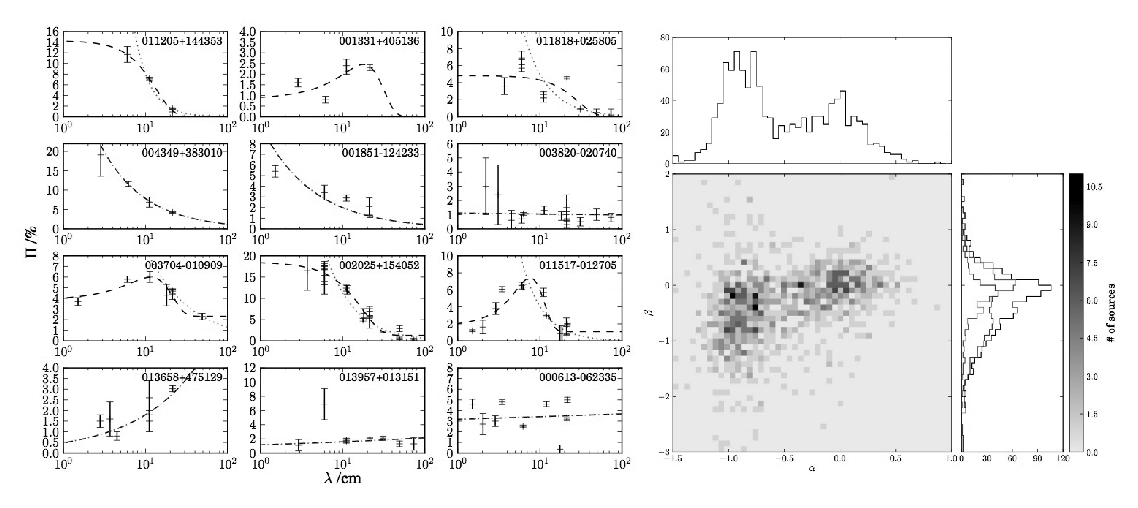
\includegraphics[width=0.9\linewidth]{magnetism/c06.s2.ss3.f1.eps}
%%%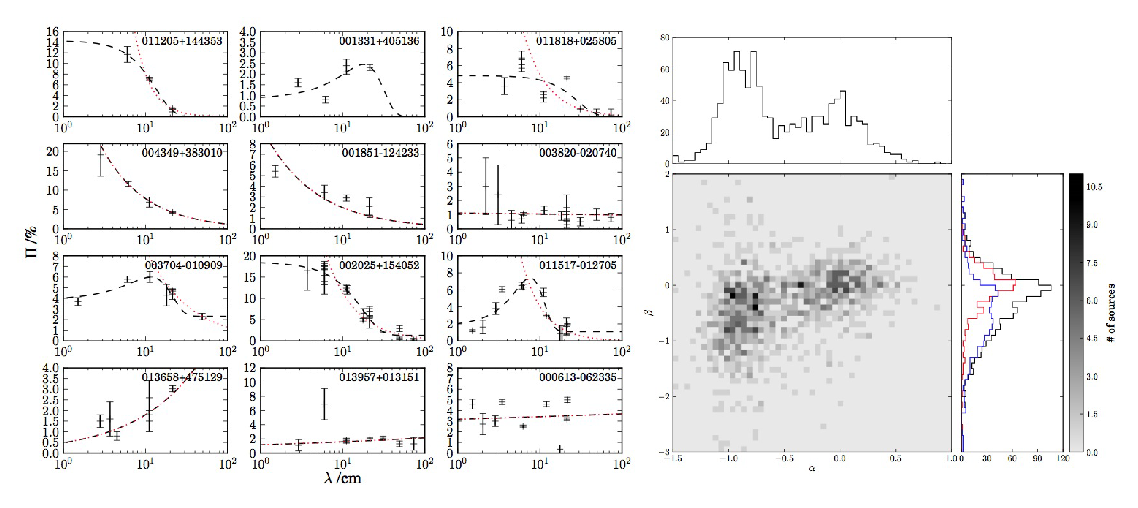
\includegraphics[width=0.9\linewidth]{magnetism/c06.s2.ss3.f1c.eps}
\end{center}
\caption{
左図:偏波率と波長の関係\citep{2014ApJS..212...15F}。破線は4つの偏波解消モデルから選ばれたベストな偏波スペクトルエネルギー分布(SED)のフィット。上段からガウス則\citep{1966MNRAS.133...67B}、冪則 \citep{1991MNRAS.250..726T}、部分ガウス則\citep{2008A&A...487..865R}、再偏波(逆偏波解消)冪則\citep{2012ApJ...747L..24H, 2012AJ....144..105H}。点線は偏波スペクトル指数を求めるのに使ったベストフィットの冪則。データの質はモデルフィットの$\chi^2$やKS-testのp-valueで分類され、左から右にかけて``accept", ``caution", ``poor"である。右図:951偏波源の電波強度スペクトル指数$I\propto \nu^\alpha$と偏波強度スペクトル指数$P\propto \lambda^\beta$の関係。
}\label{c06.s2.ss3.f1}
\end{figure}

異なる赤方偏移の偏波源を比較したり、観測データを密度や磁場強度などの物理情報に変換する計算では、観測された特性を放射とファラデー回転が起きた系に修正する必要がある(K補正)。電波強度の場合K補正は単に電波源の赤方偏移とスペクトル指数を使ったリスケーリングであるが、偏波分光では状況は複雑である。例えばAGNからの偏波は単純な波長の関数で特徴付けできない。図\ref{c06.s2.ss3.f1}は400 MHzから100 GHzの波長に渡る複数の偏波測定を含んだ951の偏波源で構成された偏波スペクトルエネルギー分布(SED)カタログの一部である\citep{2014ApJS..212...15F}。図に示すように、いくつかの偏波源は偏波解消され、また再偏波されるもの、振動するものなど様々である。ここで単一波長の偏波の測定はあまり情報に富んでおらず、広帯域データにより初めて意味のある物理がもたらされる。


%%%%%%%%%%%%%%%%%%%%%%%%%%%%%%%%%%%%%%%%%%%%%%%
\subsubsection{観測の見通し}
\label{c06.s2.ss3.sss2}

\paragraph{近傍銀河}

観測方法としては(i) 周波数:SKA1-MID band4 (2.8--5.18GHz)、(ii) 分解能:$5''$、(iii) 感度:rmsノイズは0.2$\mu$ Jy/beam (12hr)、の諸元で高分解能の偏波観測を行う。候補となるサンプルは20Mpc以内、Dec$<15^\circ$にある銀河として (i) Face-onに近い:M33, NGC300, 628, 1566, 1808, 2997, Circinus、(ii) Edge-on:M104, NGC55, 253, 3628, 4666, 4945、(iii) 棒渦巻き銀河:M83, NGC107, 1313, 1365, 1502, 1672, 2442、(iv) 不規則銀河:LMC, SMC、(v) 矮小銀河:NGC1140, 1705, 5253, IC4662、(vi) 楕円銀河(活動的でない):NGC1404, 4697を挙げる。

\paragraph{遠方銀河(深探査)}

\begin{figure}[tbp]
\begin{center}
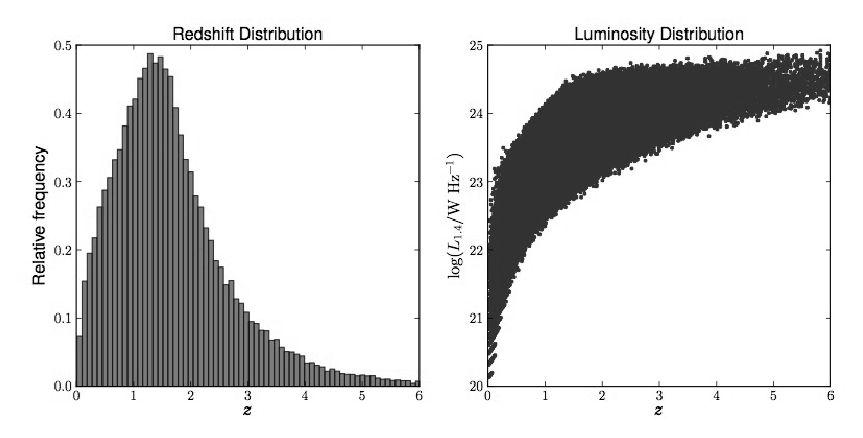
\includegraphics[width=0.8\linewidth]{magnetism/c06.s2.ss3.f2.eps}
%%%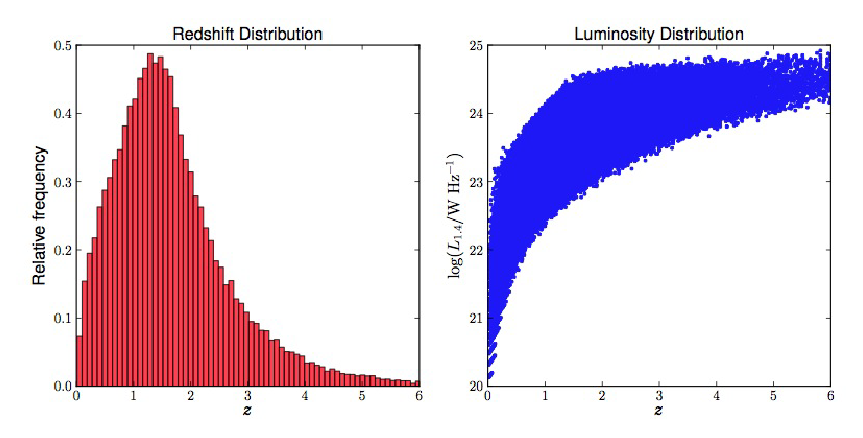
\includegraphics[width=0.8\linewidth]{magnetism/c06.s2.ss3.f2c.eps}
\end{center}
\caption{
左図:75 nJy以上の偏波強度を持った近傍円盤銀河の偏波特性を持つ通常星形成銀河の赤方偏移分布。右図:同じ銀河分布の赤方偏移と電波強度の関係。
}\label{c06.s2.ss3.f2}
\end{figure}

図\ref{c06.s2.ss3.f2}にはSKA1-MIDでポインティングあたり約100時間観測し75nJy RMSを達成した際に、10 $\sigma$以上の偏波強度を持つ銀河の赤方偏移分布である。計算は近傍渦巻銀河を考えたモデル\citep{2009ApJ...693.1392S}に基づき、近傍渦巻銀河としてSKADS S3シミュレーション\citep{2008MNRAS.388.1335W}の通常星形成銀河を適用した。ここで、高赤方偏移で偏波で受かる銀河は近傍の銀河よりかなり明るい銀河の性質を教える。なぜなら探知している銀河は電波光度関数の明るい側の端に位置するからである。なお、天体を分類するためやプラズマ密度を測るための他の波長での深探査が必要で、光赤外で選ばれた高赤方偏移銀河の偏波を探ることを前提としている。

\paragraph{遠方銀河(広帯域観測1)}

達成に必要なのは(i) 視線上の異なるタイプのファラデー回転と偏波解消の間の縮退を解くための広帯域、(ii) 偏波と可視光分光データの両方が手に入る意味のあるサンプルを累積するための高感度と高速サーベイ、(iii) 可視光スペクトルの位置に対応する背景偏波の部分を切り出すための高い角度分解能、である。すべての条件を満たすためにはSKAを建設する以外にない。おそらく一緒に実行できるHI吸収線サーベイや次世代の可視光・赤外観測装置(4MOST, WFIRST, LSST, Euclid)と組み合わせると、幅広い赤方偏移に渡って通常銀河のガス、乱流、磁化、そして空間的広がりの全貌をつかめるだろう。

\paragraph{遠方銀河(広帯域観測2)}

偏波源の静止系での偏波特性を決めるためには、幅広い波長に渡る連続的な偏波データで較正された完全な偏波SEDが要求される。従来の研究は周波数範囲が荒く、個々のデータ点は異なる時期・望遠鏡・角度分解能の別のサーベイに由来するたけ一貫性がない。数も十分とはいえない。SKAの広帯域偏波観測は様々なタイプのK補正を間違いなく正確に行うのに適し、偏波とファラデー回転を両方特徴づけそして幅広い赤方偏移に渡って偏波源を比べるために役立つ多数の偏波SEDサンプルをもたらすだろう。スペクトル指数やスペクトルの曲率・折れ曲がりなどの詳細な研究も容易になるだろう。一例を図\ref{c06.s2.ss3.f1}に示す。この951の偏波源カタログは電波強度スペクトル指数$\alpha\sim 0$の光学的に厚いコアタイプと$\alpha\sim -0.7$の光学的に薄いローブタイプがあることを示した。そしてその偏波源情報である$\alpha$に対して偏波強度スペクトル指数$\beta$が依存しているため、偏波解消も主に偏波源周辺で起こっている可能性を示唆している。


%%%%%%%%%%%%%%%%%%%%%%%%%%%%%%%%%%%%%%%%%%%%%%%
%%%%%%%%%%%%%%%%%%%%%%%%%%%%%%%%%%%%%%%%%%%%%%%
\subsection{AGN・ジェット磁場}
\label{c06.s2.ss4}

%%%%%%%%%%%%%%%%%%%%%%%%%%%%%%%%%%%%%%%%%%%%%%%
\subsubsection{科学的課題}
\label{c06.s2.ss4.sss1}

\paragraph{RL-AGN、RQ-AGNと放射}

RL-AGNからの放射は、大部分が相対論的ジェットからの非熱的放射で説明できる。低光度のRL-AGNは線幅の広い輝線が弱い傾向にあり、RIAFとの関連を指摘する研究がある。一方、RQ-AGNからの放射は、電波以外の波長帯は熱的放射が優勢で降着円盤と考えられているが、電波帯の起源は議論が分かれる。最近の観測からは、$z\sim 1.5-2$のRQ-AGNは電波放射の全てが星形成によると仮定して矛盾しない。RQ-AGNと星形成銀河の星形成率は推定されているが、RL-AGNはジェットの寄与が大きいため星形成率を見積もる事が難しい。

\paragraph{ブレーザーと放射}

ブレーザーのエネルギー散逸の多くは逆コンプトン散乱によってGeV光子として放出されるが、その散逸がブラックホール近傍のsub-pcスケールなのかもっと遠いのか不明である。1990年代にEGRET観測は、GeV光子はsub-pcスケールのbroad line regionで生じていることを示した。しかし、近年の電波からGeV帯までの他波長モニタリングでは、いつくかの場合においては数pc領域で生じていることを示唆している。VLBI観測からは、ガンマ線フレアが生じると同時に電波コアから超光速成分の放出が起きている事が示唆されている。

\paragraph{RL-クエーサーと放射}

クエーサージェットの強いX線放射領域(ノット)は、電波や赤外、光学でも光っていることが知られている。X線は逆コンプトン散乱によって放射していると考えられている。これは、電子はローレンツ因子$\gamma \sim 10-100$を持ち、ジェットはkpcスケールでも相対論的な運動をしている事を示唆する(群ローレンツ因子$\Gamma \sim 10-20$に相当)。X線放射が2次加速電子からのシンクロトロン放射と考えると超相対論的な速度である必要はないが、電子のエネルギーは少なくとも30 TeVになる必要がある。Fermi衛星の観測によって3C273に関しては逆コンプトン散乱によるモデルが否定された。

\paragraph{FRI、FRII電波銀河と放射}

ジェットのパワーは狭輝線の輝度と相関があり\citep{1991Natur.349..138R}、降着率と相関している事が分かっている。例えば、強いジェットは高い質量降着率に対応している。ゆえにFRIはRIAFが根源で弱いジェットがあり、FRIIは光学的に厚い円盤が根源で大規模なジェットがあると考えられる。X線連星では光学的に厚い円盤と薄い円盤の状態遷移が知られており、この二つが共存する銀河が将来的に見つかるかもしれない。そしてその変化には磁場形状の変化が関係しているかもしれない。

\paragraph{ジェットの形成と変動}

AGNジェットの引き金として、ブラックホール回りの星間ガスや潮汐破壊された星の物質降着が指摘されており、その降着に磁場は重要な役割を担うだろう。ジェットのエネルギーは\cite{1977MNRAS.179..433B}過程による回転ブラックホールからの引き抜きで説明できるが、Blandford \& Znajek過程のみではジェットを収束できないため、何か他の収束機構が必要である。\cite{1982MNRAS.199..883B}は幾何学的に薄い降着円盤からの非相対論的な磁化風の自己相似解を求め、その後相対論的なモデルに拡張されている。磁気回転不安定性(動的ダイナモ理論)のモデル\citep{1991ApJ...376..214B}では、降着円盤を貫くポロイダル磁場からトロイダル磁場が作られ、ポロイダル方向のポインティングフラックスが生じ、ポロイダル磁場に沿ったプラズマ加速で電流が生成され、ポインティングフラックスが運動エネルギーに変換される。観測から、事象の地平面の近傍での磁場強度は数千ガウスと示唆されており、降着円盤磁場からそのような磁場をどのようにブラックホールを貫いて作るかが課題である。また、中心エンジンからどのくらいの距離で、ジェットがポインティングフラックス優勢から運動エネルギー優勢に変化するべきか、粒子加速が研究途上のため理解できていない。AGNジェットから年単位の激しい時間変動が観測されている。ブラックホール質量やスピンは短時間では変化しない事から、磁場が変動しているのだろう。この変動も上手く説明できなければならない。

\paragraph{ジェットの速度場と粒子加速}

低光度のFRIジェットはkpcスケールで減衰し外層境界で速度勾配が大きくなるが、パワフルで細いkpcスケールのジェットの速度勾配はあまり観測されていない。弱磁場プラズマの場合、強い流体力学的衝撃波が粒子加速の主因で、それはべき乗のエネルギースペクトルを作りうる。最近のPIC計算などによる研究から、相対論的衝撃波による粒子加速でべき乗分布は再現されるが、その冪は上流のプラズマ速度や磁場強度、磁場形状などに強く依存する事がわかってきている。現実でも、FR I、FR II、そして両方の特徴を兼ね備えたAGNの存在は、周辺環境がジェット光度に影響を与えていることを示唆している。一方、強磁場プラズマの場合は磁気リコネクションや磁気乱流による相互作用が粒子加速の主因となるだろう。X線や$\gamma$線観測は宇宙線電子のスペクトルを与え、最も優勢となる放射領域とその環境に制限を与える。しかし、X線領域に対応する宇宙線電子は放射冷却などによりその分布が変化し、また$\gamma$線は$\gamma \gamma$吸収やペア生成によってスペクトル形状が変化する。その点SKAは、電波領域で放射が優勢な、比較的低エネルギーの、加速されたばかりの若い宇宙線電子を探ることができる。

\paragraph{ジェット磁場のトポロジー}

理論研究からはトロイダルないしヘリカルな磁場構造が示唆されている。観測的には3C273ではヘリカル磁場構造が示唆されているが、検証には高感度と高分解能の両立が必要なため、確認例は乏しい。ヘリカル磁場は横方向の強度に非対称性があるため、系統的な横方向のファラデー回転勾配が期待される。3C120や3C273では最も良いpcスケールの観測結果が得られており、前景は少なく、ジェット自身のファラデー回転を見ている事が示唆されている。なお、もしヘリカルな磁場構造があるとして、それがジェット形成時の磁場を反映しているのか否かは不明である。もし観測されたトロイダル磁場がジェット形成時の磁場であるならば、系統的で対称なファラデー回転の勾配が期待される。

\paragraph{フィードバック}

銀河団ガスの放射冷却時間は宇宙年齢より短い。そのためエネルギーを失ったガスは銀河団のポテンシャル中心に落下しうる。クーリングフローとも呼ばれるそのガスの流れは$10-100~{\rm M_{\odot}/yr}$と推定されたが、X線観測によって、銀河団中心には期待される冷たいガスは無いことが示された。強いクーリングフローに対抗する加熱機構は、銀河の活動性や銀河団衝突の衝撃波などが考えられる。AGNの相対論的ジェットは中心ブラックホールからMpcスケールの銀河団ガスにまで大量の運動エネルギーを放出しうる。近年の観測によって、銀河団中心部に見られる電波ローブと呼ばれる広がった放射は、マッハ数1--2程度の衝撃波に囲まれていることがわかってきた。銀河団中心のcD銀河ジェットアウトフローとの関係が示唆される。

%%%%%%%%%%%%%%%%%%%%%%%%%%%%%%%%%%%%%%%%%%%%%%%
\subsubsection{観測の見通し}
\label{c06.s2.ss4.sss2}

\paragraph{SKA1の見通し}

SKA1では (i)AGNジェットの宇宙論的研究、(ii)円偏波を用いた大まかなジェット組成、(iii) 電波の弱いAGNの何千個に及ぶ撮像からAGNのジェットパワーの本質的な違い、(iv) 速度・放射率・磁場構造から検討したジェットの3次元的な物理量、(v) ストークスパラメータの観測からジェットの周辺環境の予測、(vi) 銀河団の偏波観測と合わせたジェットと周辺環境の相関の理解、などの理解が進むと期待される。SKA1-MIDのBand3を用いて多数のRQ,RL AGNを観測し、明るい天体をSKA1-VLBIのBand3と5で追観測しジェットと星形成を区別することで、星形成率を議論できる。またSKA1-VLBIのBand5で多数のpcスケールの直線に伸びたジェットを観測・分解する事で、(a) ファラデー回転の勾配はジェット軸に直交するか (b) RM synthesisによって放射プラズマと熱的成分の混合の証拠は見つかるか (c) 視線方向に進むジェットと反対向きのジェットとの間で勾配に異なる傾向はあるか、などの疑問に答えられる。AGNがどこで光りエネルギーを散逸しているかは、ジェットの形成や収束モデルに多大な影響を与えるため重要な研究課題である。高感度・高分解能の観測でしか解決できず、SKAのような大望遠鏡が必要である。

\paragraph{円偏波の観測}

円偏波(ストークスV)の観測から磁場強度の直接観測が可能となり、ジェットによって伝搬する実際の磁気フラックスを測定できる。この他、陽電子-陽子比などの組成比、低エネルギーカットオフに関する情報も得られる。円偏波は非常に弱く(ストークスIの0.1-1\%)変動が激しいため、他の3つのパラメータ(ストークスI, Q, U、直線偏波P)と比べ観測が非常に難しい。その点SKA1の高感度、広帯域の観測は円偏波測定に理想的な装置である。現在、円偏波が測定されるAGNは少ない($<100$)ので、SKA1では1--20 GHzのサーベイ観測を行う。円偏波で明るい天体を発見したら、SKA1-VLBIの追加観測によって放射領域を特定し、理論との比較からジェットの物理パラメータ(強度、組成、磁束)を決定できるだろう。

\begin{figure}[tbp]
\begin{center}
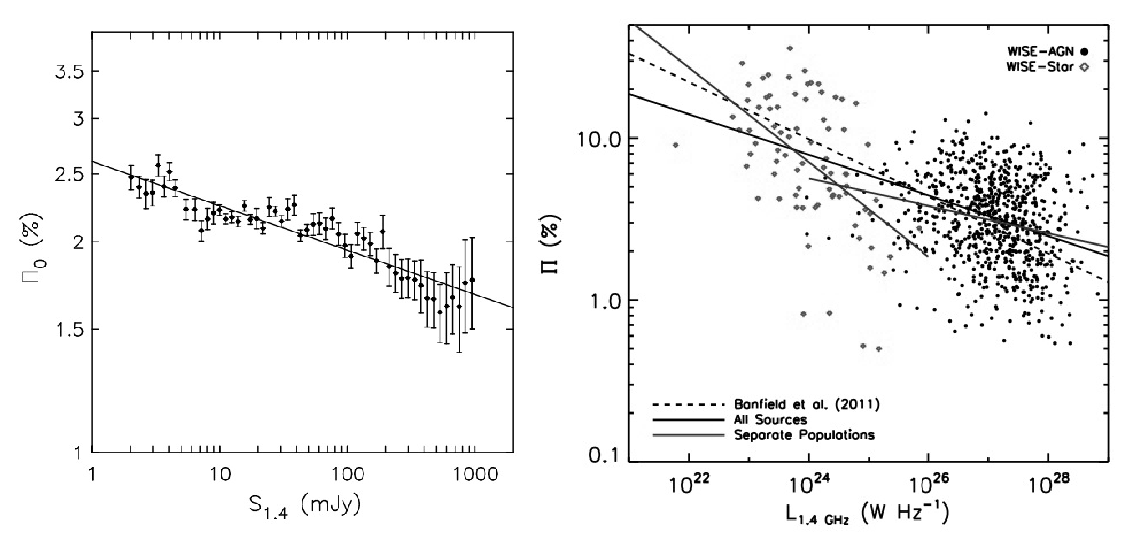
\includegraphics[width=0.9\linewidth]{magnetism/c06.s2.ss4.f1.eps}
%%%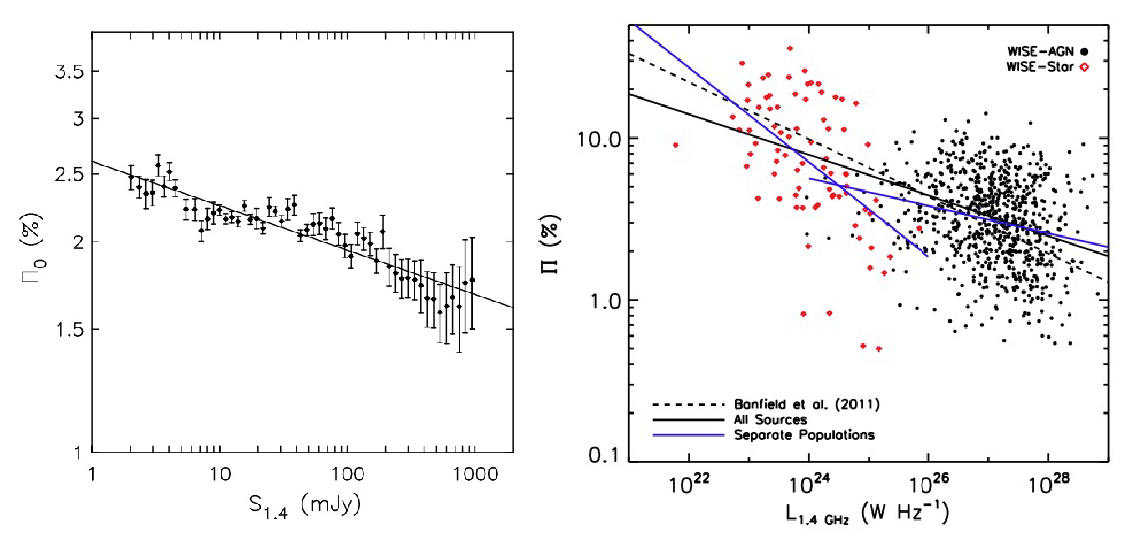
\includegraphics[width=0.9\linewidth]{magnetism/c06.s2.ss4.f1c.eps}
\end{center}
\caption{
系外偏波源の電波強度と偏波率の関係。左図はNVSSのスタッキング結果\citep{2014ApJ...787...99S}。右図はNVSSデータに赤外線対応(赤:近傍早期型銀河、黒:遠方AGN)のあるものを取り出した結果\citep{1404.1638}。近傍星形成銀河の偏波率は遠方AGN偏波源よりも高い。
}\label{c06.s2.ss4.f1}
\end{figure}

\paragraph{深探査1}

異なる赤方偏移で大量のソースの偏波率を測ることは磁場の構築を時間の関数として確かめることを可能にし、そのばらつきを起こしうるブラックホールへの物質降着の変動の情報も与えるだろう。深い観測で$z \sim 5-10$のAGNジェットからの電波放射のスペクトルを研究できる可能性がある。究極的には、宇宙最初のAGNとその超巨大ブラックホールは何かを極高赤方偏移にさかのぼり調べることが重要であり、SKAの大集光力ではじめて可能となる。ここで、近傍から赤方偏移10にかけて宇宙論的平均密度は1000倍になるため、ジェットは母銀河を打ち破るのがどんどん難しくなる。そのような系はGPS(GHz Peaked Spectrum)ソースとして近傍宇宙で知られ、高密度ないし若いジェットの環境に対応する\citep{1998PASP..110..493O}。母銀河内のジェットの閉じ込めは銀河と中心ブラックホールの共進化、ジェット物質を通じたその磁化、AGNと銀河間物質の相互作用に強い示唆を持つだろう。SKAで100 nJy RMSの観測を果たせば、エディントン光度で光っている$z\sim 8$までの通常銀河の中のブラックホール環境を観測しうる。

\paragraph{深探査2}

NVSSの180万の系外電波源のうち14 \%は有意に(3$\sigma$以上で)偏波シグナルを示していた\citep{1998AJ....115.1693C, 2003AJ....125..465H}。偏波の特性は$z\sim 3$まで赤方偏移にあまり依存していない一方で、偏波率と電波強度には逆相関関係がみられる\citep{2002A&A...396..463M,2007ApJ...666..201T}。図\ref{c06.s2.ss4.f1}には最新の結果を示す。逆相関関係は、高偏波率電波源については、可視光形態・赤方偏移・サイズ・電波強度に対して強い依存性を持たない\citep{2010MNRAS.409..821S}が、低光度偏波源に向かって緩やかになる\citep{2014ApJ...787...99S}。逆相関関係は偏波源の磁場構造の変化を示唆する。逆相関関係を説明する解、radio-quiet AGNの割合ないしFR II--FR I遷移の変化が指摘されている。

\begin{figure}[tbp]
\begin{center}
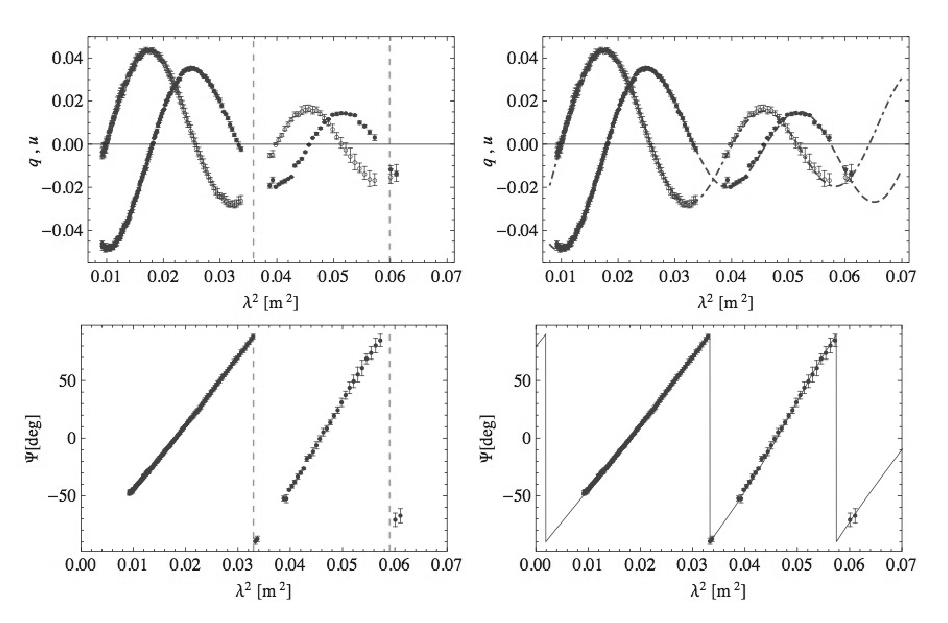
\includegraphics[width=0.8\linewidth]{magnetism/c06.s2.ss4.f2.eps}
%%%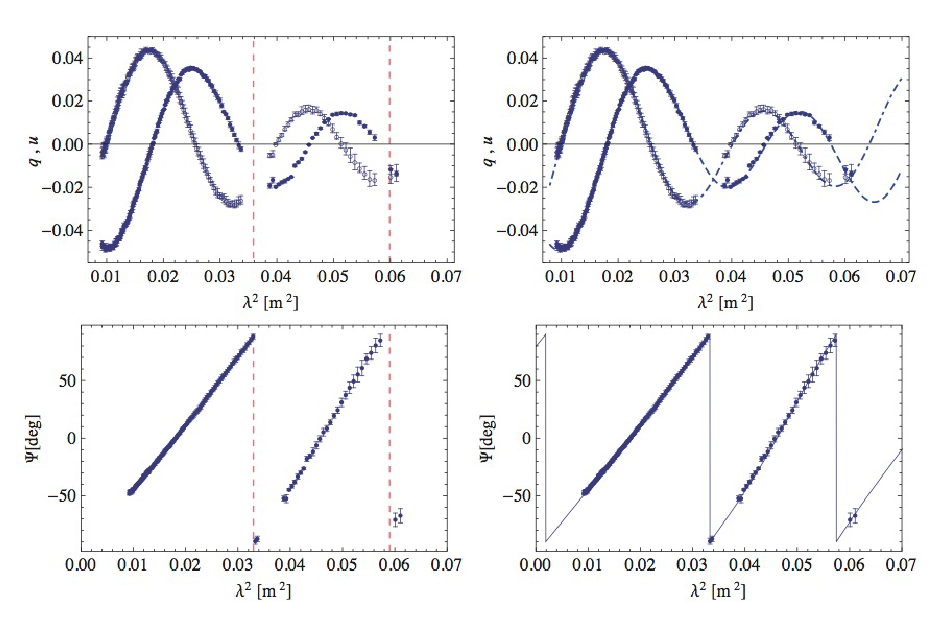
\includegraphics[width=0.8\linewidth]{magnetism/c06.s2.ss4.f2c.eps}
\end{center}
\caption{
クェーサーPKS B1610-771の1.1 GHzから3.1 GHzまでの偏波データ\citep{2012MNRAS.421.3300O}. 上図:波長の2乗に対するストークスq(=Q/I, 白丸)とu(=U/I, 黒丸)。左側の破線は1.4 GHzを中心とする350 MHz帯域の観測で得られるレンジ。右側で全バンド幅のデータは2つのRMを持つモデルでフィットされる。下図:波長の2乗に対する偏波角。
}\label{c06.s2.ss4.f2}
\end{figure}

\paragraph{広帯域観測1}

近傍に限る僅かなサンプル数ではあるが、AGNの電波ローブの周辺環境との相互作用の様子が明らかになってきた。しかしながら、電波ローブの中の熱的ガスの存在についてはほとんどが上限値しか求められていない\citep{1985ApJ...297...84S, 1987MNRAS.228..557L, 2004ApJ...604L..77K}。最近、空間的に分解された分光偏波とRMグリッドを組み合わる新しいアプローチが提案され\citep{2013ApJ...764..162O}、近傍電波銀河Centaurus Aの電波ローブの内側に熱的電子密度$\sim 10^{-4}$ ${\rm cm^{-3}}$の存在を示した。これはAGNジェットとローブで年200太陽質量のガスを牽引したことになり、銀河間物質との相互作用よりもホスト銀河自身に由来するガスと支持される。この結果は、新しいCentaurus AのX線観測にも支持されて、AGNアウトフローとフィードバックを研究する新しい方法を示した。

\paragraph{広帯域観測2}

図\ref{c06.s2.ss4.f2}には明るい遠方クェーサー PKS B1610-771の観測結果を示す\citep{2012MNRAS.421.3300O}。偏波角と波長の2乗のプロットは線形依存性からずれていること、ストークスパラメータと波長の2乗のプロットが強度一定の正弦波パターンを示さず偏波率は波長の2乗について定数でないこと、そして上記の振る舞いは狭帯域で観測しても分からないことが分かる。例えば、1.4 GHzを中心とする350 MHz帯域の観測\citep{2004NewAR..48.1003G, 2004NewAR..48.1289B}では、$0.036 \ge \lambda^2~({\rm m^2}) \ge 0.060$ をカバーするが(赤点線)、これでは+135~${\rm rad~m^{-2}}$のRMをもつ単一の前景と解釈され、偏波源が持つだろう興味深い性質を認識し理解する可能性はない。それに対して、右図では2つの空間的に離れて異なるRMをもつ成分モデルでデータをフィットした。このシンプルなモデルは観測とよい一致を示し、+107~${\rm rad~m^{-2}}$と+79~${\rm rad~m^{-2}}$のRMをもつ2つの偏波したノットがあるという結論を導く。この例のように、SKAの広帯域によって、AGNからの電波ローブの中や周辺の熱的ガスの分布を包括的に探査することが可能になる。


%%%%%%%%%%%%%%%%%%%%%%%%%%%%%%%%%%%%%%%%%%%%%%%
%%%%%%%%%%%%%%%%%%%%%%%%%%%%%%%%%%%%%%%%%%%%%%%
\subsection{銀河団磁場}
\label{c06.s2.ss5}

%%%%%%%%%%%%%%%%%%%%%%%%%%%%%%%%%%%%%%%%%%%%%%%
\subsubsection{科学的課題}
\label{c06.s2.ss5.sss1}

\paragraph{起源と進化}

近年のファラデー回転の観測、ならびにそれぞれ50例を超えている電波ハロー・レリックの観測により、磁場のモデル化が進んでいる。その一方で、銀河団磁場の起源や増幅機構については、例えば原始磁場と構造形成ダイナモの組み合わせ\citep{2008Sci...320..909R}やAGNおよび銀河風\citep{2000ApJ...541...88V}によるものなど諸説あるが(\S \ref{c06.s1.ss6}参照)、その詳細は不明である。理論と観測との比較が効果的な解決手段であり、双方のさらなる精密化が不可欠である。

\paragraph{磁場の構造}

基本的には、銀河団磁場は銀河団ガスの乱流の影響をうけて乱流磁場と考えられるが、AGNからのアウトフローや電波レリックなどでは整列した磁場もあるだろう。RMや電波ハローの偏波観測は磁場の空間パワースペクトルを知るのに重要である。大スケールと小スケールのどちらかに磁場エネルギーがあるかにより、観測される偏波の空間的なパターンが違うと予想されるからである。実際、いくつかの銀河団について、偏波観測から磁場のパワースペクトルが議論されている。RMについては乱流はコルモゴロフ的ではないかという示唆がある\citep{2008A&A...483..699G}。電波ハローについては、一般的に観測される偏波は弱いので、偏波が観測されにくい小スケールに磁場のエネルギーがあると考えられる。しかし、偏波観測から磁場や宇宙線を議論する場合、ビーム内での平均化や偏波解消の影響も考慮する必要がある。

\paragraph{モデルの構築}

近年のファラデー回転の観測により銀河団のモデル化が進んでいる。例えばガス分布については球対称ベータモデルか宇宙論的シミュレーションのデータを用いる。磁場モデルについては、パワースペクトルがコルモゴロフ則に従うランダムガウシアンとし、また局所的な磁場強度はガス密度のべき乗に比例すると仮定する。また最近では、銀河団形成の宇宙論的なMHDシミュレーションも試み始めている。観測結果を宇宙論的な MHD シミュレーションと比較することは有用である。さまざまな磁場の初期条件で計算をし、得られた銀河団中の磁場と実際の観測データを比較することで、銀河団磁場の起源について迫ることができるであろう。このように銀河団のガス分布および磁場、それに加えて偏波源のモデルを考えて、模擬RM観測データを作る。SKAによる観測が始まる前でも、シミュレーションデータを利用した模擬観測を行うことで、観測プランを立てることができる。例えば、X線では見分けにくいマッハ数$\sim $1--2の弱い衝撃波で、磁場の圧縮に伴う偏波が観測できるかどうか議論することができる。

\paragraph{RM構造} 

1.4 GHzで1 $\mu$Jyの感度、角分解能$1.6''$を仮定すると、1平方角あたり315個の偏波源が検出されると予想される(図\ref{c06.s2.ss1.f1})。典型的銀河団とされるかみのけ座銀河団によく似たモデル銀河団を観測すると、背後に50個の偏波源を検出するだろう。VLAによるかみのけ座銀河団の結果が7個だったので大幅な増加である。その結果、RMの半径方向の構造を再現できるようになり、また磁場のモデルパラメーターの縮退も解けるようになると予測される。また、現実的な銀河団の密度分布として宇宙論的シミュレーション\citep{2010NewA...15..695V}で作った銀河団を用いた結果、RMプロファイルに銀河団の力学状態に応じた違いが見られることが分かった。銀河団ガス中の衝撃波をRMで検出できるかについても調べてみた。宇宙論的シミュレーションデータ中の銀河団で、衝撃波面を通る方向とそうでない方向とでRMプロファイルを比較した。その結果、衝撃波付近でのRM増加の兆候を見ることができた。なお、このシミュレーションでは磁場の進化は取り入れていない。また衝撃波付近での密度上昇にともなう磁場上昇しかはいっていない。実際にはそれ以外の効果でもっと磁場増幅が起きている可能性が高く、今回よりは衝撃波を見つけやすくなっている可能性が高い。

\paragraph{電波ハロー} 

電波ハローの大きさはMpcにもなるが、表面輝度は小さく(1.4 GHzで$\sim \mu \rm Jy~arcsec^{-2}$)、スペクトルは急($\alpha>1$)である\citep{2012A&ARv..20...54F}。磁場の大きさは$\sim 0.1$--$1\:\rm \mu\: G$と見積もられている。ハローの表面輝度のゆらぎは磁場の構造を反映していると考えられる。各銀河団での電波ハローのシンクロトロン放射の分布と銀河団ガスからのX線放射の分布との比較が行われている。巨大で形が整った電波ハローについてはシンクロトロン放射の分布とX線放射の分布が一致していることが多い\citep{2012A&ARv..20...54F}。一方、不規則な形をした電波ハローについては、シンクロトロン放射の分布とX線放射の分布が大きくずれていることが多く、その場合ハローの大きさは小さいことが多いようである\citep{2012A&ARv..20...54F}。この違いは銀河団衝突と関係している可能性がある。例えば、ハローの大きさが小さい銀河団は銀河団衝突の初期段階にあり、磁場がまだ乱流などによりよくかき混ぜられておらず、結果として初期に持っていた大きいスケールでの不規則な形を保存しており、シンクロトロン放射の分布もそれを反映しているのかもしれない。

%%%%%%%%%%%%%%%%%%%%%%%%%%%%%%%%%%%%%%%%%%%%%%%
\subsubsection{観測の見通し}
\label{c06.s2.ss5.sss2}

\paragraph{SKA1の見通し}

SKA1で定義されている性能は、現在の観測装置の全ての性能指標を基本的に上回る。感度の向上により、偏波源の個数が限られ比較対象するためのサンプルが足りなかった問題は大幅に改善される。RMグリッドで現状の観測装置では判別不可能な銀河団磁場構造の詳細に迫ることができる。現状では困難な$10^{13-14}$太陽質量の小規模銀河団でも中心磁場強度やRM構造の解析を可能にするだろう。SKA1の初期科学運用(感度約50\%)で得られる結果は偏波源の個数に依存する。小規模銀河団や衝撃波については厳しそうであるが、大規模銀河団については十分に有望だろう。高分解と広視野という両立の難しい要求は、SKA1では1秒以下の分解能(X線望遠鏡Chandraと同程度)で度スケールの視野(銀河団を網羅するサイズ)を与えので、銀河団の研究に非常に適している。同時観測帯域も向上するため、不足していた宇宙線スペクトルを精密に決定するための電波・偏波のスペクトル情報も得られるだろう。

\paragraph{SKA2の見通し}

SKA2では感度で10倍、視野で20倍良くなる予定である。最悪の場合(SKA1と偏波源の検出数は変わらない)でもSKA1と同じことを短時間でできるはずである。分解能も向上する分だけ、より小スケールの磁場構造を探ることができる。


%%%%%%%%%%%%%%%%%%%%%%%%%%%%%%%%%%%%%%%%%%%%%%%
%%%%%%%%%%%%%%%%%%%%%%%%%%%%%%%%%%%%%%%%%%%%%%%
\subsection{宇宙大規模構造磁場}
\label{c06.s2.ss6}

%%%%%%%%%%%%%%%%%%%%%%%%%%%%%%%%%%%%%%%%%%%%%%%
\subsubsection{科学的課題}
\label{c06.s2.ss6.sss1}

\paragraph{銀河間磁場の理論予測}

 $\Lambda$CDM宇宙は銀河団やフィラメントなどの蜘蛛の巣構造を予言する。銀河団は $T > 10^7$ Kの熱いプラズマを含んでいる一方で、フィラメントは中高温銀河間物質と参照される$10^5$ K $< T < 10^7$ Kのプラズマで満ちている。プラズマは磁化していると期待される。種磁場の多様な過程が指摘されており、またその種磁場はさらに圧縮や乱流ダイナモ、銀河物質の流出などで、階層的宇宙構造形成の中で増幅されうる\citep{2012SSRv..166....1R,2012SSRv..166...37W}。RMは蜘蛛の巣構造の銀河間物質を研究するための主要なツールである。銀河団では$B \sim 1 - 10\ \mu$Gが明らかにされてきている。それと比べて、フィラメントの磁場のRM研究はわずかであり、主にRMが小さいことが原因である。フィラメントでの銀河間磁場は宇宙論的シミュレーションに基づけば \citep{2008Sci...320..909R}おそらく$B \sim 1-100$ nGくらいだろう。

\paragraph{銀河間磁場のRMの理論予測}

\begin{figure}[tbp]
\begin{center}
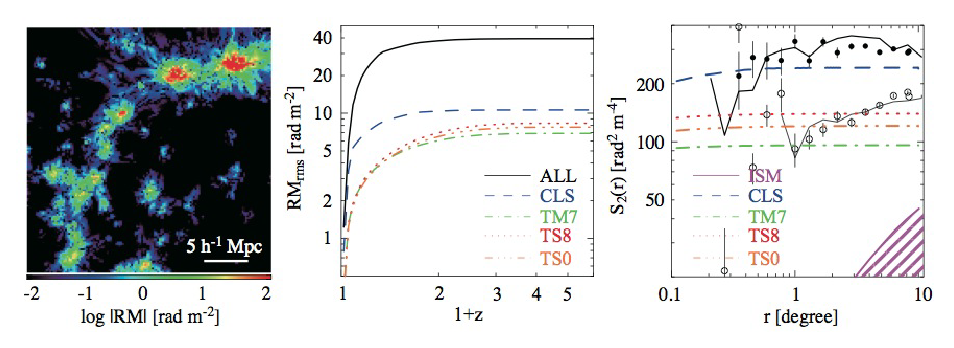
\includegraphics[width=1.0\linewidth]{magnetism/c06.s2.ss6.f1.eps}
\end{center}
\caption{左:深さ$100$ $h^{-1}$Mpcの近傍宇宙のRMマップ\citep{2010ApJ...723..476A}。中:赤方偏移最大5まで積分したRMのrms値\citep{2011ApJ...738..134A}。異なる銀河団の除去モデルが異なる色で示されている。右:RMの2次構造関数。黒丸\citep{2010ApJ...714.1170M}と線\citep{2011ApJ...726....4S}は$\sim 900$平方度の
北(filled, thick)と南(open, thin)銀極の観測値. 紫の領域は極方向の天の川銀河のRMのあり得る強度を示している\citep{2013ApJ...767..150A}。
}\label{c06.s2.ss6.f1}
\end{figure}

図\ref{c06.s2.ss6.f1}には銀河間磁場のモデルに基づいたRMのシミュレーション結果を示す。RMのrms値は一つのフィラメントあたり $\sim 1$~${\rm rad~m^{-2}}$であり(図\ref{c06.s2.ss6.f1}左)、赤方偏移で数までの複数のフィラメントを通過したRMのrms値は数 ${\rm rad~m^{-2}}$に達する(図\ref{c06.s2.ss6.f1}中)。興味深いことに、そのようなRMは観測されたRMの系外からの寄与の見積もり$\sim 6-15$~${\rm rad~m^{-2}}$ \citep{2010MNRAS.409L..99S,1209.1438v2}と同程度になる。ここで2次構造関数を定義する。
\begin{equation}
S_n(r)=\langle|RM(\vec{x}+\vec{r})-RM(\vec{x})|^2\rangle _{\vec{x}}
\end{equation}
$r=|\vec{r}|$は角距離でデータ$x$に対して平均値を求める。2次構造関数はパワースペクトルと同様に空間相関の様子を定量化し、離散的に分布する観測データでも容易に計算できるので、観測的研究ではよく用いられる指標である。シミュレーションはフィラメントの銀河間磁場は角度スケール$\sim 0.1^\circ$以上で$\sim 100$ rad$^2$ m$^{-4}$の強度を持ったフラットなRM2次構造関数を示す(図\ref{c06.s2.ss6.f1}右)。天の川銀河の寄与が最小な銀緯の高い方向で、銀河磁場はずっと小さくかつ冪を持つ構造関数をその角度スケールでは作るべきである\citep{2013ApJ...767..150A}。高銀緯方向の観測された構造関数は観測されたフィラメントの銀河間磁場起因のそれと一致しており\citep{2010ApJ...714.1170M,2011ApJ...726....4S}、フィラメントの銀河間磁場が重大な寄与をしていることを指摘している。


%%%%%%%%%%%%%%%%%%%%%%%%%%%%%%%%%%%%%%%%%%%%%%%
\subsubsection{観測の見通し}
\label{c06.s2.ss6.sss2}

\paragraph{SKA1の深探査}

高銀緯方向で銀河団の外側の方向というのがフィラメントの銀河間磁場を深RM探査で探るために選ばれるべきである。さらに他のRM寄与を取り除く必要もある。天の川銀河のRMはハイパス・フィルターで十分に取り除けるだろう\citep{2014ApJ...790..123A}。偏波源と介在系のRMは強く偏波解消したソースを取り除くことで避ける事が可能であろう。というのも、それらのRMは深探査の $\sim 1''$ビーム (赤方偏移0.5で6.1~kpc)内で強いビーム偏波解消を示すべきであり、一方で銀河間磁場のRMはそのスケールでは小さなRMの勾配しかなくあまり偏波解消を示さないだろう。

\paragraph{統計的なアプローチ}

100nJy以下の感度の深探査は、偏波源を選別しても1平方度あたり100個程度の偏波源を提供するだろう。そのようなデータは$r > \sim 0.1^\circ$の構造関数を十分な精度で解き明かすことができ\citep{2014ApJ...790..123A}、銀河間磁場のRMを抽出することを可能にする。

\paragraph{ファラデートモグラフィー}

銀河間磁場のRMはファラデースペクトルにおいて背景と前景の間のファラデー深度のギャップとして見つかりうる\citep{2014PASJ...66...65A}。数${\rm rad~m^{-2}}$のギャップであれば、深探査のSKA1-MID band2, band3のデータで$\sim 3\sigma$程度の優位性で探知できる\citep{2014PASJ...66....5I}。


%%%%%%%%%%%%%%%%%%%%%%%%%%%%%%%%%%%%%%%%%%%%%%%
%%%%%%%%%%%%%%%%%%%%%%%%%%%%%%%%%%%%%%%%%%%%%%%
\subsection{宇宙論的磁場}
\label{c06.s2.ss7}

%%%%%%%%%%%%%%%%%%%%%%%%%%%%%%%%%%%%%%%%%%%%%%%
\subsubsection{科学的課題}
\label{c06.s2.ss7.sss1}

\paragraph{スタック解析}

個々の天体からは強度が弱すぎて検出不可能であるような偏波を統計的に検出する手段として、偏波のスタック解析がある。スタック解析は主に系外銀河磁場やAGN・ジェット磁場の研究に役立つと期待されるが、銀河間磁場の探査にも活用しうるので、この小節で紹介することにする。スタック解析とは、別のサーベイ(例えばストークス Iパラメタによるカタログや可視光サーベイなど)によって位置が分かっている天体について、その位置を基準にシグナルを足していくという手法である。スタック解析により (i) 偏波解消の宇宙年齢に渡る進化、(ii) 矮小銀河など暗い天体の磁場の検出、(iii) 磁場の向きと他の観測量(傾斜角や銀河形態、スペクトル指数など)との関係、(iv) 周波数分解能を上げた観測、の研究が可能になると期待されている。

\paragraph{スタック解析の結果}

NVSSサンプルにおける天体一つに対しての偏波度検出限界は$S_{1.4}\gtrsim 80$ mJy程度であるが、スタック解析によってこの限界を越えることができ、暗い天体ほど偏波度が大きいという傾向が明らかに現れている(図\ref{c06.s2.ss4.f1}左)。この傾向の原因の一つとして、暗い天体ほど高赤方偏移にあり、ファラデー偏波解消の効果が小さくなるため見かけの相関として見えているのではないか、という考え方がある\citep{2002A&A...396..463M}。したがって、将来SKAの観測によって赤方偏移毎に相関をとることは重要であろう。周波数ターゲットや感度を考えると、SKA-SUR band3 (1.5-4.0 GHz), およびSKA-MID Band2 (0.95-1.76 GHz)がこの研究に適していると考えられる。ただし、HIや可視光のサーベイにより赤方偏移を特定しておく必要がある。また、偏波のスタック解析ではconfusion limitには特に気をつける必要がある。

%%%%%%%%%%%%%%%%%%%%%%%%%%%%%%%%%%%%%%%%%%%%%%%
\subsubsection{観測の見通し}
\label{c06.s2.ss7.sss2}

\paragraph{SKA1の見通し}

他に光度の小さい銀河をスタックすることにより、星生成率と磁場の間の関係を大小様々な銀河に渡って探ることできる。特に矮小銀河、星形成銀河、銀河系のような銀河で磁場の状態が異なるのかどうか、は興味があるところである。ダイナモ理論によれば、星形成からのエネルギーフィードバックによる乱流生成が磁場増幅に寄与しているはずであり、これを観測的に確かめることは重要である。特にSKAによるHIサーベイカタログは、HIと星の質量比やHIの輝線からダイナミクスやガスの状態などが同時に分かるので、この研究にとって好都合である。


%%%%%%%%%%%%%%%%%%%%%%%%%%%%%%%%%%%%%%%%%%%%%%%
%%%%%%%%%%%%%%%%%%%%%%%%%%%%%%%%%%%%%%%%%%%%%%%
\subsection{ファラデートモグラフィー}
\label{c06.s2.ss8}

%%%%%%%%%%%%%%%%%%%%%%%%%%%%%%%%%%%%%%%%%%%%%%%
\subsubsection{科学的課題}
\label{c06.s2.ss8.sss1}

\ref{c06.s2.ss7}節で見たように、広帯域の偏波観測が可能になるとファラデートモグラフィーによって磁場、熱的電子、宇宙線電子などの視線方向分布を探ることが可能になり、イメージングも組み合わせることによって天体の3次元構造の情報を得ることができる。国際SKAにおいてはこれを用いた近傍銀河の磁場の研究が議論されているが、特に次が注目されている。
(i) ファラデー回転測度と偏波度の方位角依存性など、円盤に沿った磁場の大域的構造。ダイナモ機構による予言と合うか (i) 円盤に沿った磁場が円盤に垂直な方向に関してどのように変化するか。特に銀河面に関して磁場は対称か、反対称か (ii) ハローと円盤では大域的磁場が同じ構造を持っているか、異なる構造を持っているか (iii) ハローと円盤の境界で磁場はどうなっているか。円盤からハローに乱流磁場や大域的磁場が輸送されているのか (iv) 銀河磁場は銀河風によって銀河外に輸送されているのか。またSKAでは21cm線によって中性水素の分布も観測できるため、ファラデートモグラフィーとの大きなシナジーが期待できる。
